%----------------------------------------------------------------------------
\chapter{Girvan-Newman módszer}
%----------------------------------------------------------------------------
\section{Általános tudnivaló a módszerről}

Az algoritmus elnevezése Michelle Girvan, egy amerikai fizikus, és Mark Newman, szintén egy amerikai fizikus nevéből származik. A két fizikus egy hierarchikus módszert fejlesztett ki a közösségek kimutatására komplex rendszerekben.

Az algoritmus a hálózat felépítését vizsgálja, és az élek közötti köztességi fokra épül. A köztességi fok egy érték, amely meghatározza, hogy az adott él hány legkisebb út megy át rajta. Ez az érték a forgalmat tükrözi, vagyis azt, hogy a legkisebb utak gyakori átjárhatósága mekkora. Az él közösségi fokának értéke az áthaladó összes legrövidebb út forgalmának az összege. Ez az érték segít több részre bontani a hálózatot a legforgalmasabb élek törlésével. Az így kapott részgráfok alkotják az első szintű gócokat. Ezután ezeket a részhalmazokat tovább lehet bontani, amíg minden élet törölünk.

Az általam megvalósított algoritmus három modulra épül. Az első modul az útmodul, amely a legrövidebb utak tárolásában használható, és képes az élek tárolására. A második modul az élekről tárol információkat, mint az él típusa, kezdő- és végpontja, köztességi foka és átfedési foka. Az utolsó modul azért jött létre, hogy egyik függvény visszatérési értékét tovább tudjuk adni, és ezen keresztül az éleket kezelni tudjuk.

\begin{figure}[h]
    \centering
    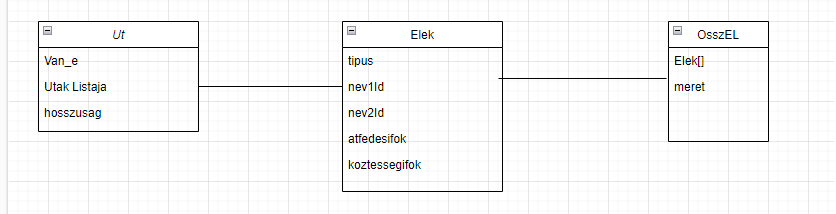
\includegraphics[scale=0.9]{images/modulok}
    \caption{Modulok}
    \label{fig:enter-label}
\end{figure}
\newpage
Modulok bemutatása után következzen a legkisebb út meghatározása :

\begin{figure}[h]
    \centering
    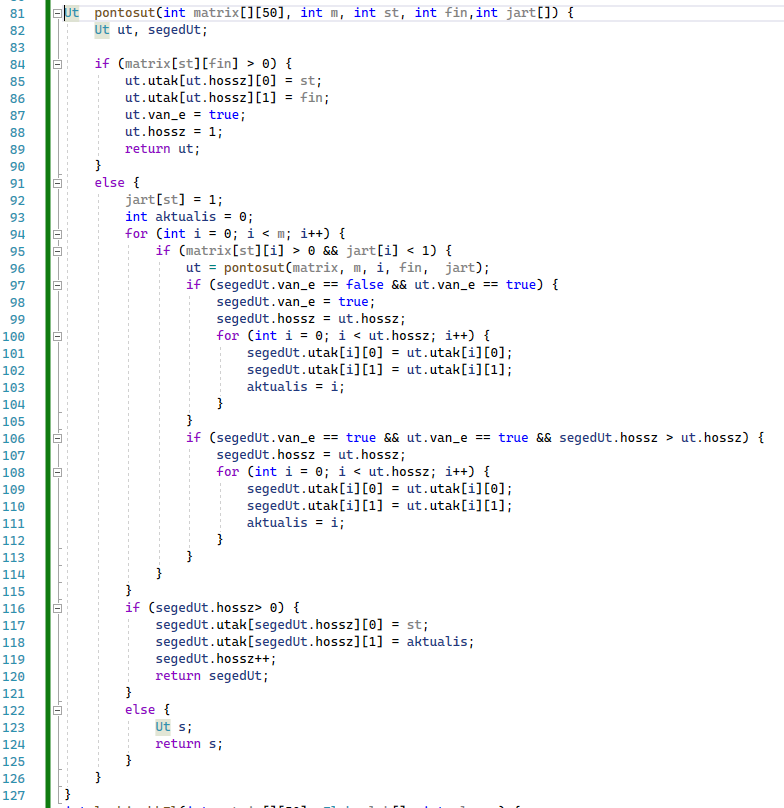
\includegraphics[scale=0.8]{images/pontosUt}
    \caption{Út meghatározására használt függvény}
    \label{fig:enter-label}
\end{figure}

Az algoritmusodban a legrövidebb utak meghatározásához szükséges az optimális útvonalak ismerete. Az élek közötti köztességi fok növelésével könnyen megtudhatod a keresett eredményt, ha pontosan ismered az irányt.

A fenti függvény meghatározza az adott út pontos éleit, és ehhez öt paramétert használ. Az első paraméter a gráf éleit tartalmazó mátrix, majd három 'int' típusú változó következik (a csúcsok száma, az indulási pont és a cél), végül pedig egy tömb, amelyben nyomon követed, hogy mely csúcsokon jártál már. A függvény első sorában létrehozol két 'Ut' típusú változót, amelyek a legjobb utat és a kapott értékeket tárolják a rekurzió során.

A függvény első ellenőrzése azt vizsgálja, hogy van-e kapcsolat az indulási pont és a cél között. Ha van kapcsolat, akkor hozzáadod az élek listáját a tárolt tömbhöz, beállítod a tömb méretét 1-re, és az "van-e ut" logikai változót igazra állítod. Ez az eset jelenti azt, amikor nem kell a függvényt újra meghívni, tehát itt véget ér a rekurzió, ha előzőleg elindult a folyamat.

A teljes függvény a rekurzióra épül, amely akkor hívja meg önmagát, ha nem kap rögtön választ, hanem tovább kell vizsgálnia. Ehhez megvizsgálod az indulási pont összes élét, hogy merre lehet továbbhaladni. Ezek az élek elvezetnek más pontokhoz, amelyekről szeretnéd megtudni, milyen messze vannak a céltól. Ez a folyamat addig ismétlődik, amíg egy vagy több megoldást találsz. Ha csak egy megoldás van, az lesz a legrövidebb út, de ha több van, akkor ki kell választanod a legjobbat. Ehhez szükséges a két változó, amelyeket az első sorban hoztál létre. Az élek listájának mérete kulcsfontosságú, mert ez döntő jelleggel befolyásolja a választ. Minél kisebb a legrövidebb út hossza, és ha valóban elértél a célhoz, annál jobb a megoldás. A ciklusban megkapod a legjobb utat, majd visszatérsz a függvényből egy kis bővítéssel. A bővítés azt jelenti, hogy hozzáadod az élt, amelyen keresztül eljutottál a legoptimálisabb szomszédhoz. Ebben az esetben növeled az élek listájának méretét, majd visszatérsz az így kapott úttal. Az így visszaadott értékek alapján beállítod az élek közötti köztességi fokot a következő függvényben.

\begin{figure}[h]
    \centering
    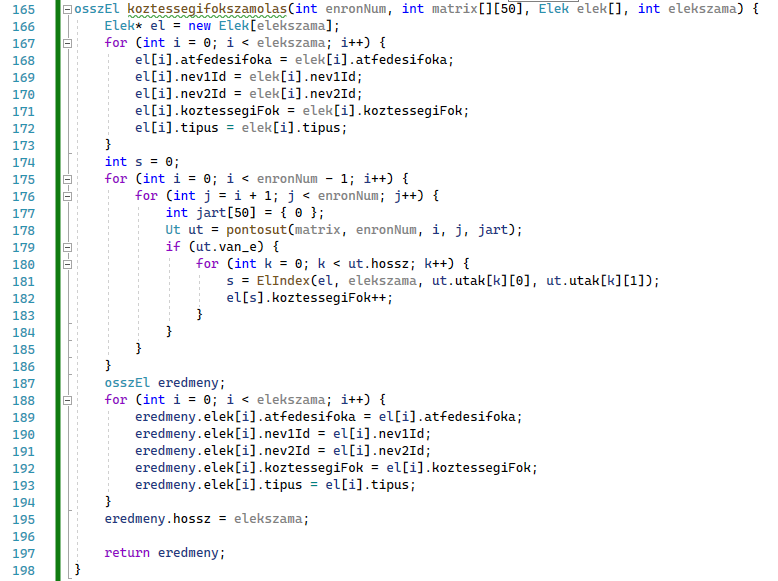
\includegraphics[scale=0.8]{images/koztessegifok}
    \caption{Köztességifok számítására alkalmazott függvény}
    \label{fig:enter-label}
\end{figure}

Ahogy látható, bejárom az összes lehetséges utat az egymásba ágyazott for ciklusok segítségével, és így meghatározom minden út pontos lépéseit. Ezeket az utakat aztán egy segédfüggvény (ElIndex) által feldolgozom, hogy növeljem az utakban előforduló élek köztessegi fokának számát. Ez a növelés akkor történik, ha az aktuális pontok között van út, mert a törlések és a komponensekre való szétesés megakadályozza, hogy minden pont között út létezzen. A köztessegi fok kiszámítása után az eredeti él listát visszatérítem, de a köztessegi fokokat átírom.

A következőkben bemutatom a Girvan-Newman módszer megvalósítását, amely segítségével meghatározom, hogy a legnagyobb azonos köztessegi fokkal rendelkező élek törlése során milyen gyorsan esik szét a gráf izolált pontokra.


\begin{figure}[h]
    \centering
    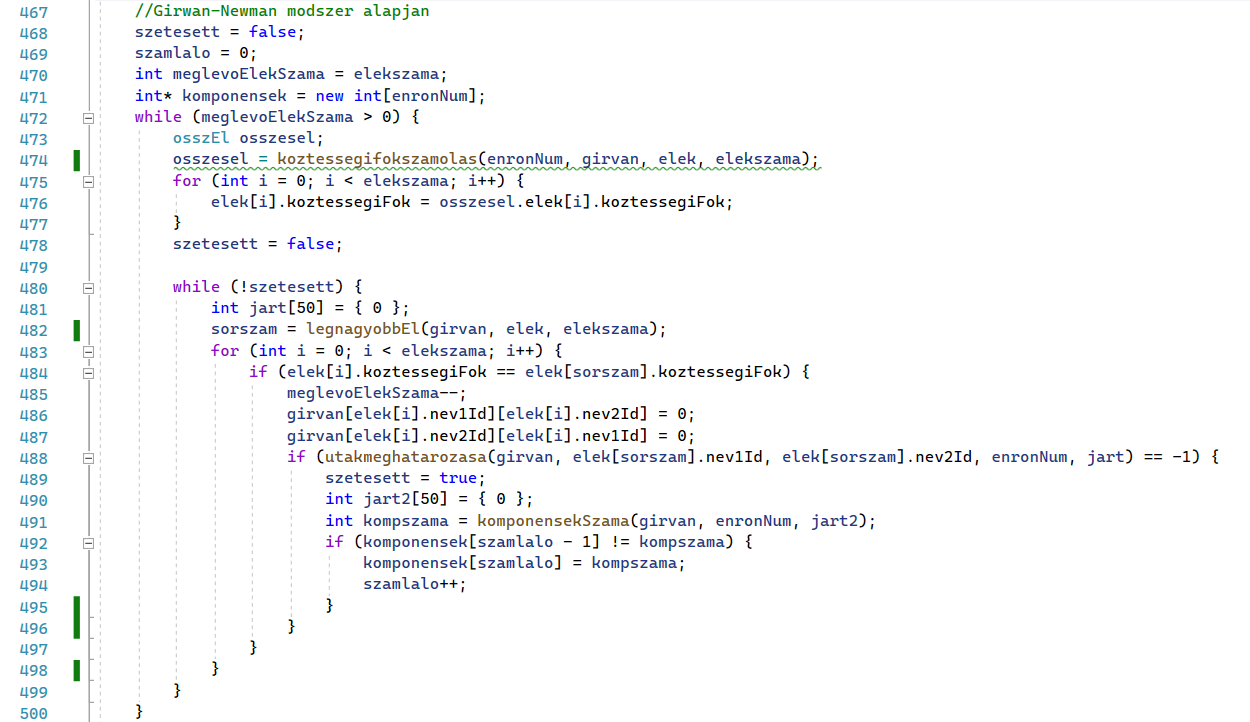
\includegraphics[scale=0.8]{images/girvan}
    \caption{Girvan-Newman módszer}
    \label{fig:enter-label}
\end{figure}

A fenti kódrészletben több egymásba ágyazott ciklus segítségével valósítom meg a műveleteket. Számolom a megmaradt éleket, amelyeket kitörlés esetén nullázok a girvan nevű mátrixon keresztül. A 488. sorban ellenőrzöm, hogy a törlés után van-e még út a törölt él két pontja között. Ha nincs, akkor biztosan változik a komponensek száma, amit később egy bejárás segítségével megszámolok és visszatérítek. Ha változik a komponensek száma, akkor visszalépek a kódrészlet elejére, újra számolom a köztessegi fokokat, majd ezt ismétlem addig, amíg elfogynak az élek.

Ezután felmerült bennem a kérdés, hogy vajon a súlyok szerinti élek törlése során nem szétesik-e hamarabb a gráf izolált csúcsokra. Ennek vizsgálatára elvégeztem a súlyok szerinti törlést csökkenő és növekvő sorrendben is. Minden művelet hasonlóan működött a Girvan-Newman algoritmushoz, hasonló ciklusokkal dolgoztam, és az eredmények is hasonlóak voltak, kis eltéréssel. A következő ábrákon látható eredmények rámutatnak arra, hogy a Girvan-Newman algoritmus a leggyorsabb módszer az összes él törlésére. Ugyanakkor, ha a súlyok kisebb szórásúak lennének, akkor véleményem szerint a gráf hamarabb szétesne a súly szerinti törlés esetén.

A következő lépésben a szoftver megjelenít egy kis adatvizualizációt, amely szemlélteti a hálózat kapcsolatainak törlés általi szétesését.
\begin{figure}[h]
    \centering
    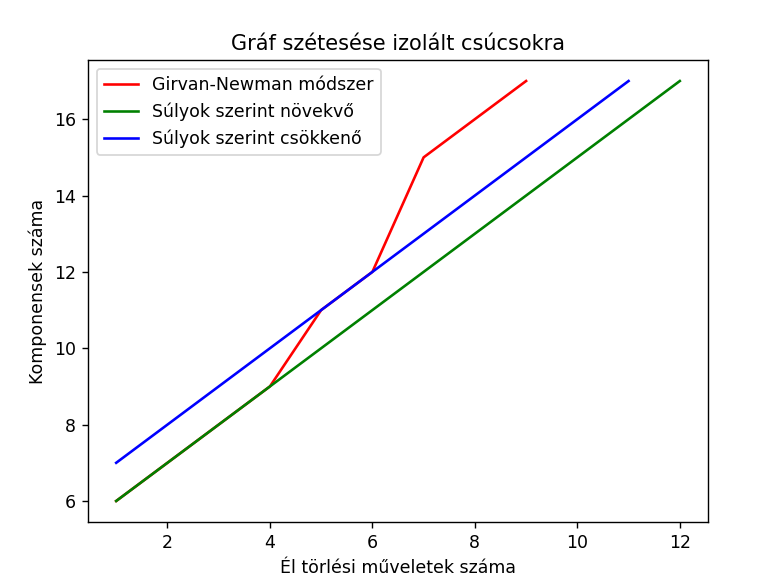
\includegraphics[scale=0.7]{images/hasonlitas}
    \caption{Összehasonlítás eredményének ábrázolása}
    \label{fig:enter-label}
\end{figure}


\begin{table}[h]
	\centering
	\begin{tabular}{ | l | c | c | c | c |}
		\hline 
		\textbf{Módszer} & \textbf{ciklusok száma} & \textbf{első éltörlés után}  \\
		\hline
		Girvan-Newman & $ 9 $ & $ 6 $  \\
		\hline
		Súlyokkal növekvő & $ 12 $ & $ 6 $ \\
		\hline
		Súlyokkal csökkenő & $ 11 $ & $ 7 $  \\
		\hline
		
	\end{tabular}
	\caption{Mérési eredmények  $ n = 17 $ csúccsal való tesztelésre.}
	\label{tablazat1}
\end{table}

A Girvan-Newman algoritmus a leggyorsabbnak bizonyult ebben az esetben, ahogy az összehasonlító ábrán is látható. Emellett bemutattam az egyes törlési események során készült állapotokat is.

A vizualizációs program lehetőséget nyújt arra, hogy válasszunk az 3 algoritmus által generált törlési események között, így kirajzolhatjuk a súlyok szerinti csökkenő vagy növekvő sorrendben bekövetkező változásokat.

Az alábbiakban megjelenítek egy állapotot, amelyet a súlyokkal való törlési művelet során generáltam:

\begin{itemize}
    \item  Az első három ábrán látható a Girvan-Newman módszer lépései által generált aktuális gráf. Ezek közül három ciklusos törlést mutatok be: az kezdeti állapotot, majd egy törlést és végül hét törlést követő állapotot. A fenti táblázatban is látható, hogy kilenc törlés után a gráf teljesen izolált csúcsokra bomlik. A két törlés azt jelzi, hogy a komponensek száma kettővel növekedett.
    \item  A második két ábrán a súlyok szerint növekvő sorrendben történik az élek kiválasztása és törlése.
    \item A táblázatban is látható, hogy a súly szerinti csökkenő és növekvő módszer nem dolgozik egyformán. Ha nem vesszük figyelembe a törlési módszer legfontosabb tulajdonságát, akkor azt gondolhatnánk, hogy a gráfban ugyanannyi különböző értékű él van, tehát mindegy, hogy lentről felfelé vagy fentről lefelé haladunk a súlyokkal, mindig ugyanannyi különböző súlyú él lesz. Úgy tűnhet, hogy nincs különbség a két módszer között. Azonban itt jön a fordulat, mert csak akkor lépünk tovább egy új lépésre, ha a törlések során a komponensek száma növekszik. Ezért a csökkenő és növekvő sorrendben történő módszer eredménye nem lesz azonos. Csak bizonyos speciális esetekben lesznek az eredmények azonosak, például ha az élek súlyai azonosak, vagy ha minden különböző súlyú él törlése több komponenst eredményez.      
\end{itemize}

\begin{figure}[h]
    \centering
    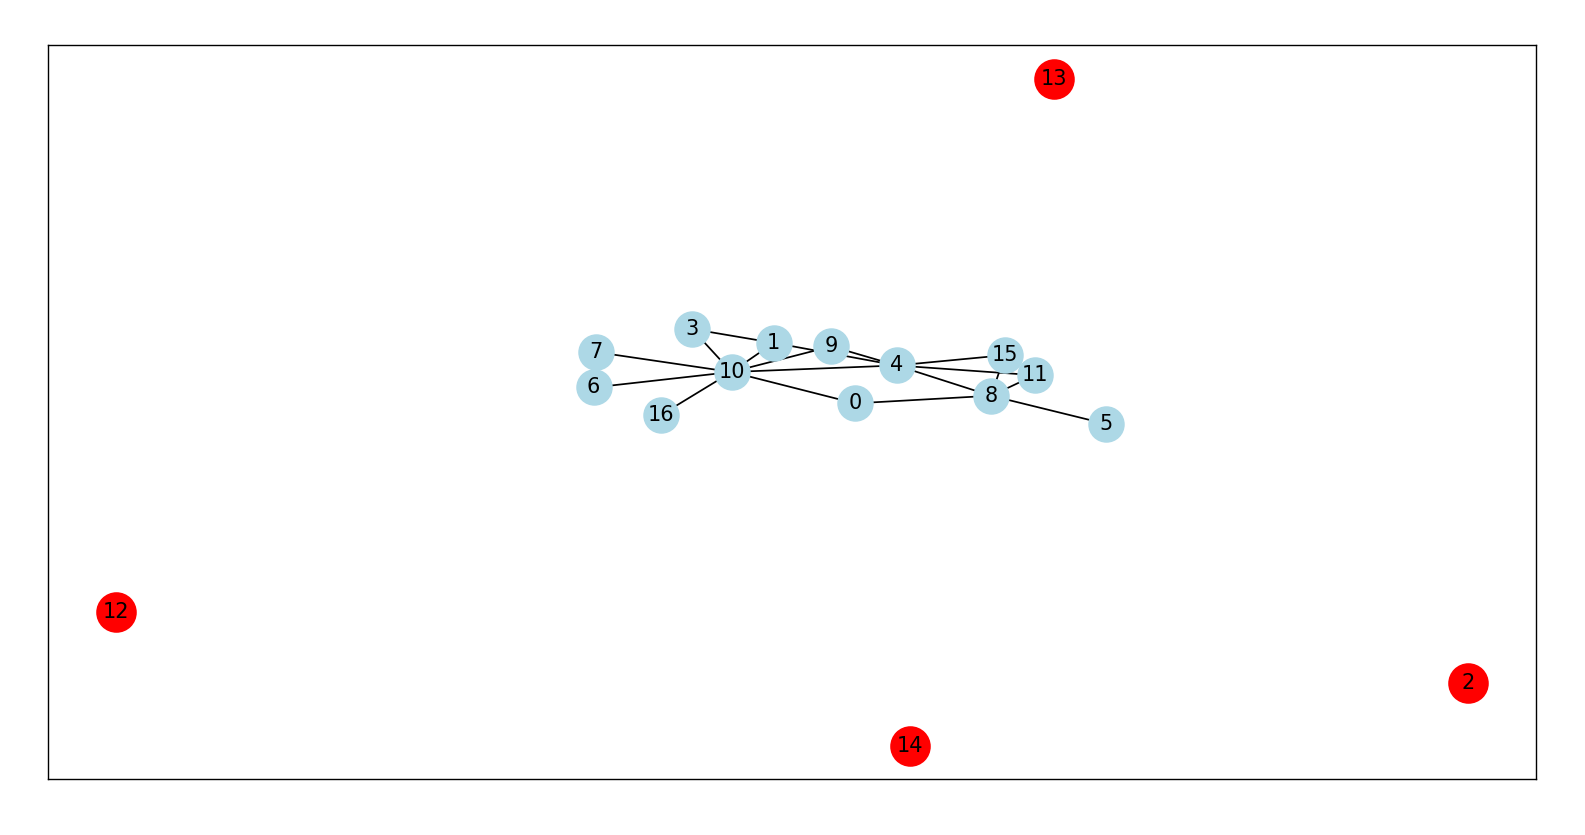
\includegraphics[scale=0.4]{images/girvan1lep}
    \caption{A gráf törlések előtt}
    \label{fig:enter-label}
\end{figure}


\begin{figure}[h]
    \centering
    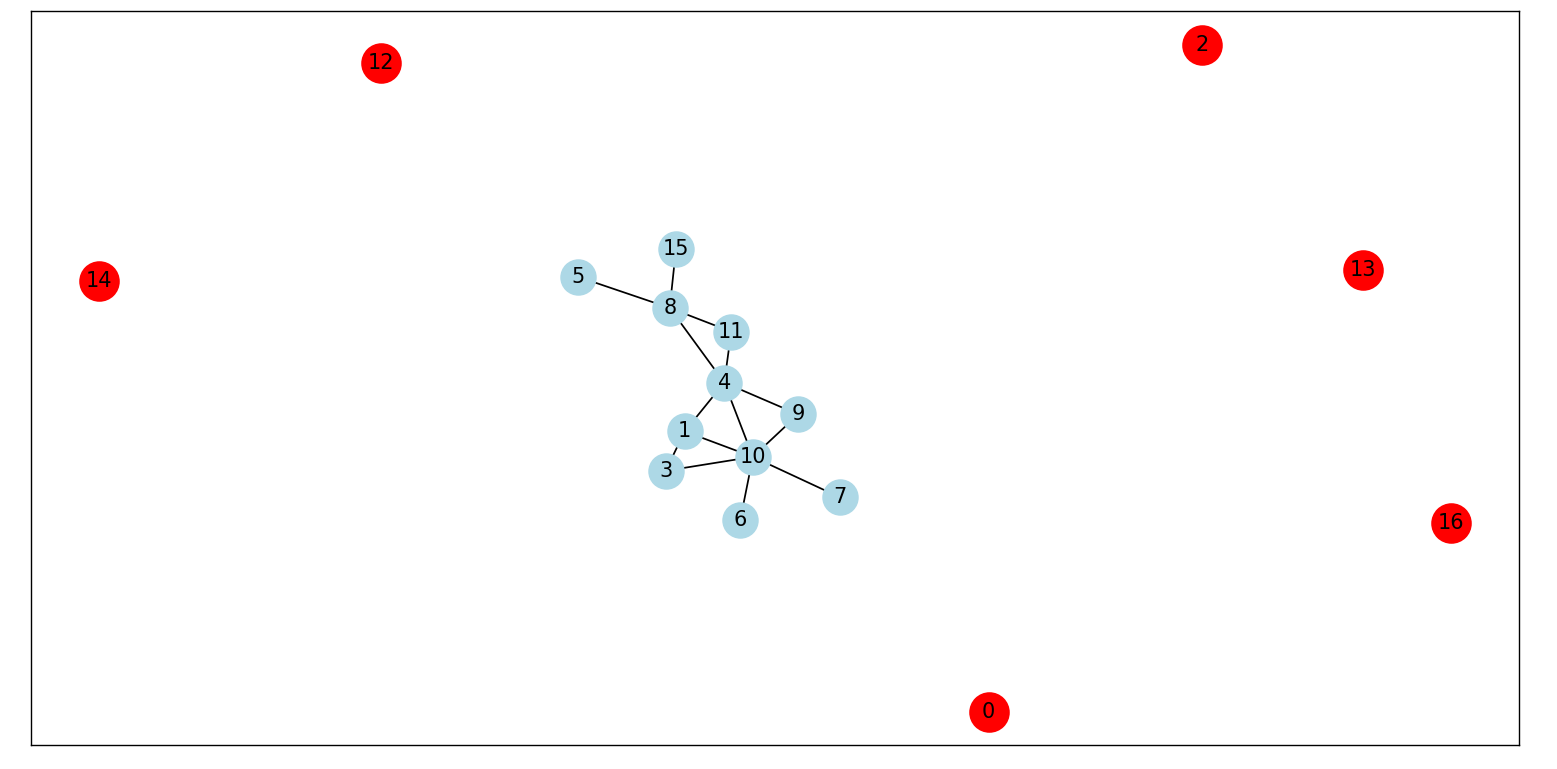
\includegraphics[scale=0.4]{images/girvan4lep}
    \caption{A gráf 2. Girvan-Newman módszerrel való törlés után }
    \label{fig:enter-label}
\end{figure}


\begin{figure}[h]
    \centering
    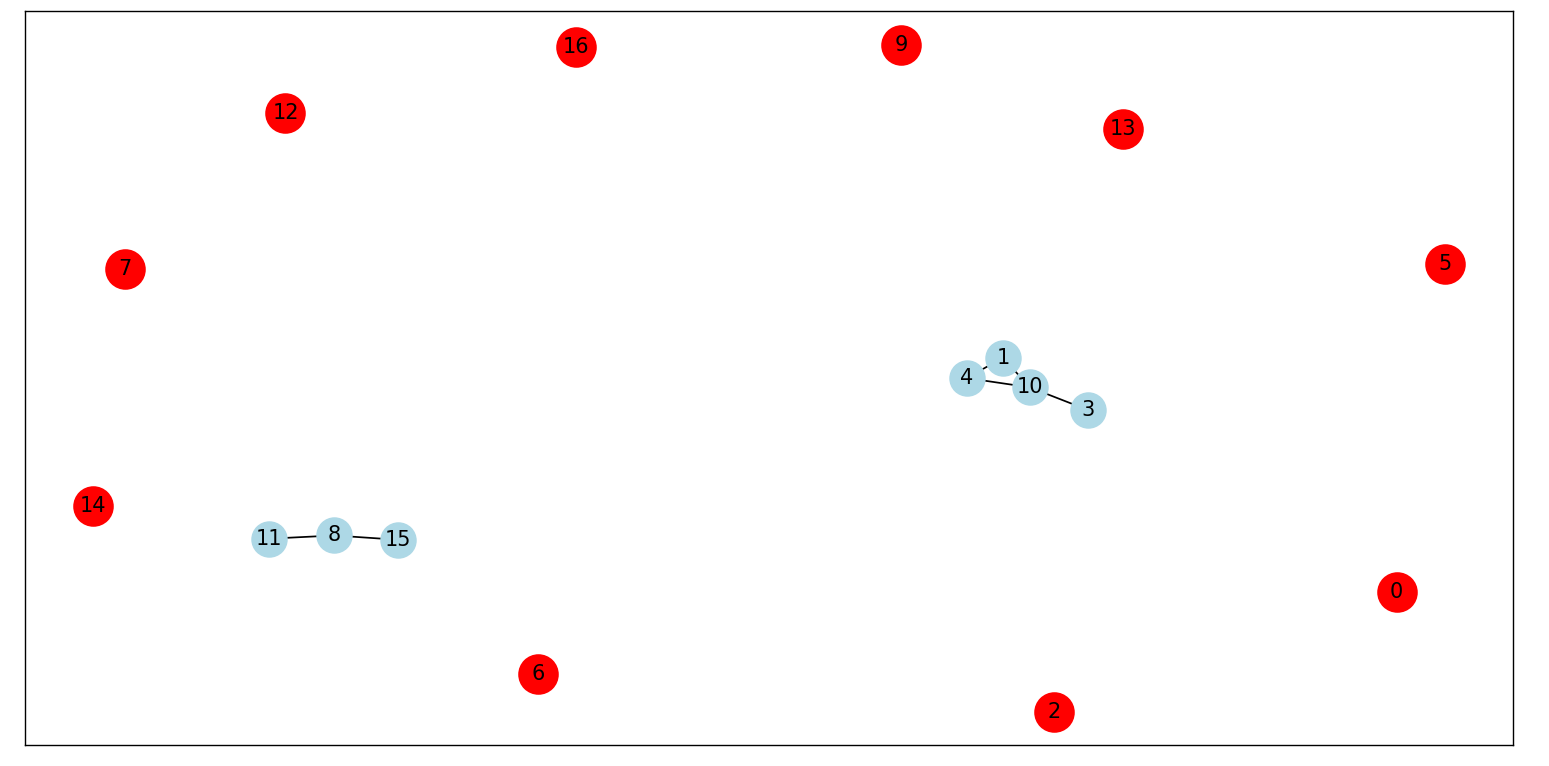
\includegraphics[scale=0.4]{images/girvan7lep}
    \caption{A gráf 7. Girvan-Newman módszerrel való törlés után}
    \label{fig:enter-label}
\end{figure}






\begin{figure}[h]
    \centering
    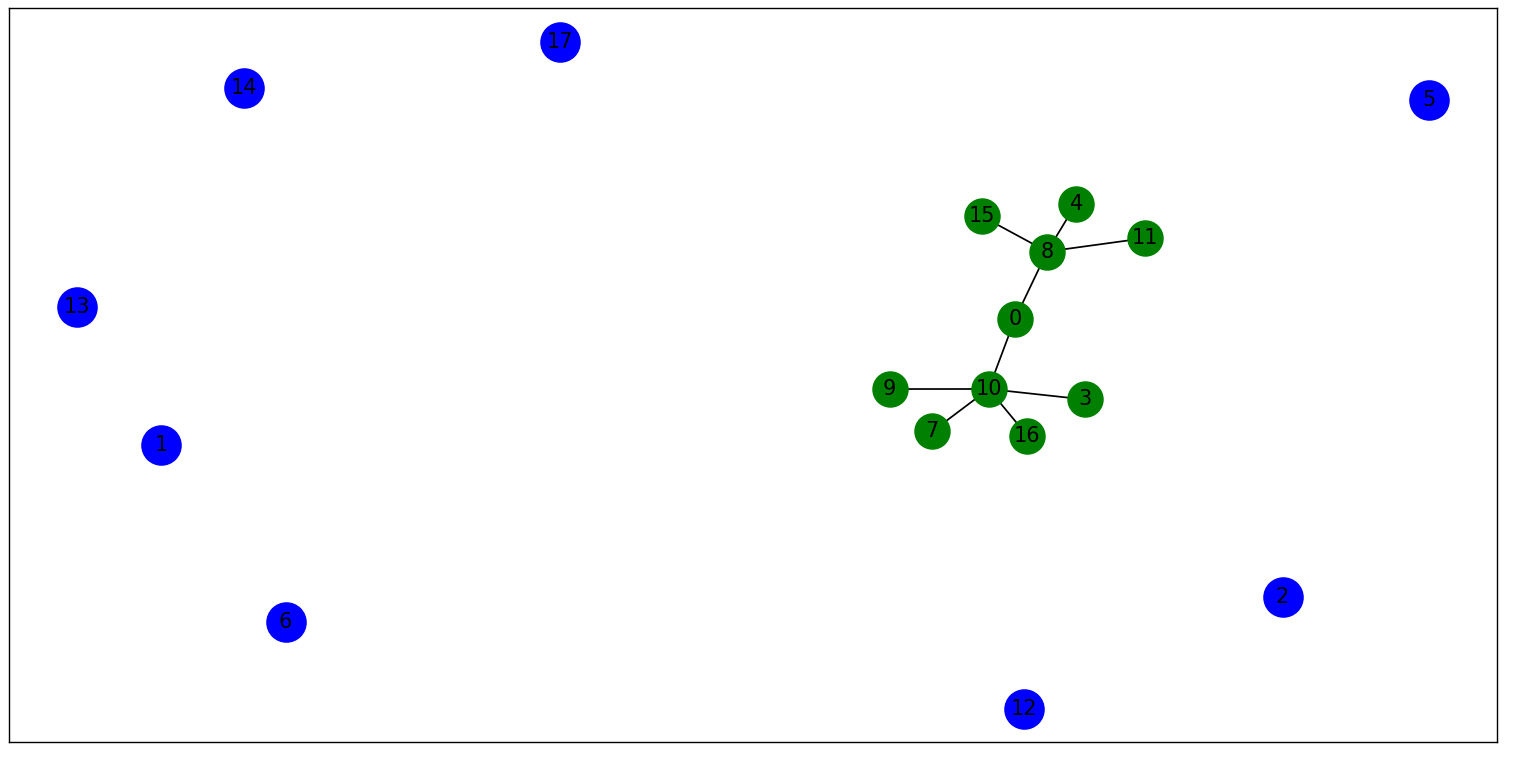
\includegraphics[scale=0.4]{images/suly5}
    \caption{A gráf 4 törlés után}
    \label{fig:enter-label}
\end{figure}


\begin{figure}[h]
    \centering
    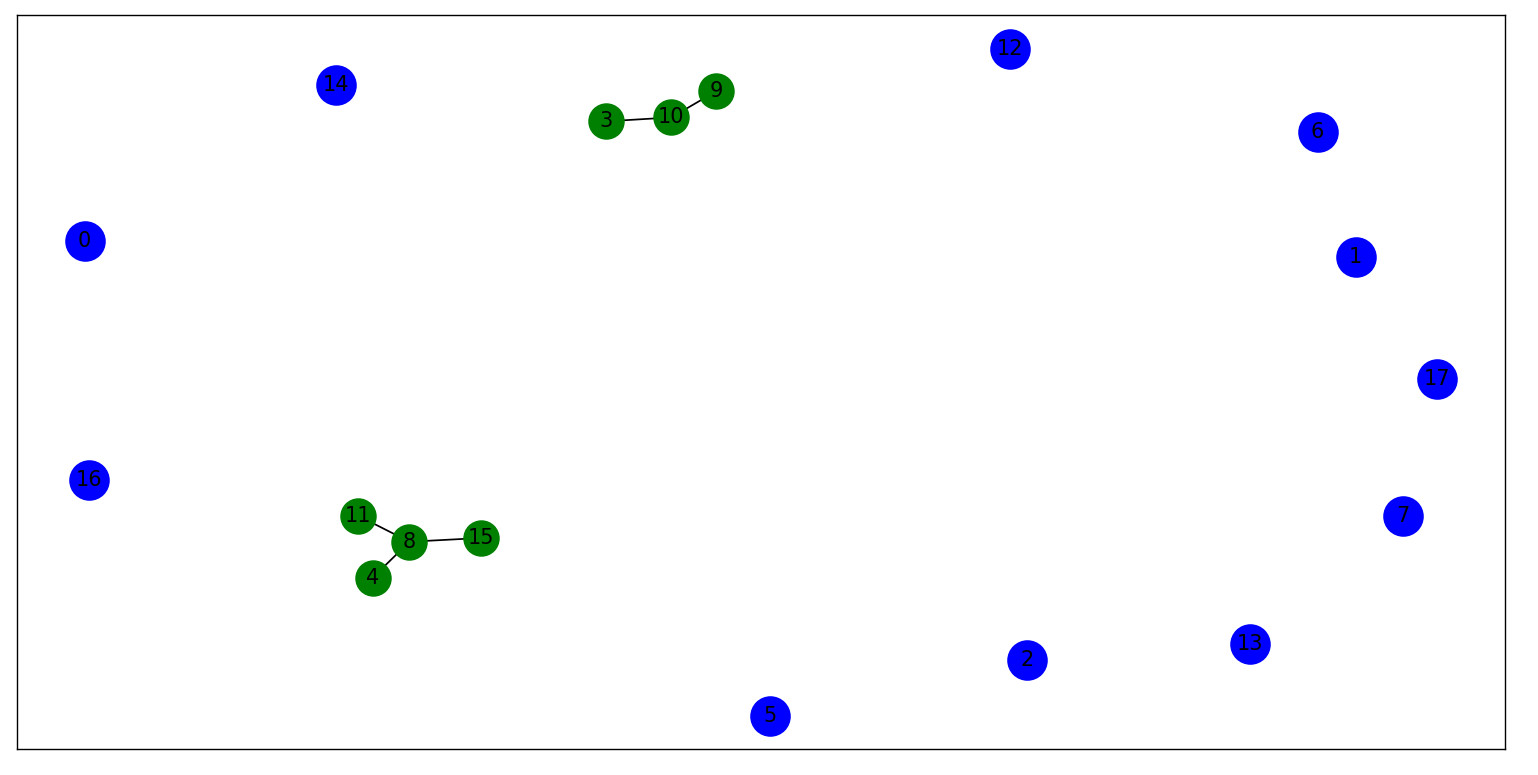
\includegraphics[scale=0.4]{images/suly9}
    \caption{A gráf 8 törlés után}
    \label{fig:enter-label}
\end{figure}



